\documentclass[12pt]{article}

\usepackage[utf8]{inputenc}
\usepackage[T1]{fontenc}
\usepackage{graphicx}
\usepackage[a4paper, left=2.5cm, right=2.5cm, top=3cm]{geometry}
\usepackage{setspace}
\usepackage{amsmath, amssymb, amstext}
\onehalfspacing

% for bash script highlighting
\usepackage{listings}

\lstdefinestyle{BashInputStyle}{
  language=bash,
  basicstyle=\small\sffamily,
  numbers=left,
  numberstyle=\tiny,
  numbersep=3pt,
  frame=tb,
  columns=fullflexible,
  linewidth=0.9\linewidth,
  xleftmargin=0.1\linewidth
}

\newcommand*{\Package}[1]{\texttt{#1}}%

%%%%%%%%% TITLE %%%%%%%%%%%%%%%%%%%%%%%%%%%%%%%%%%%%%%%%%%%%%%%%%%%%%%%%%%%%%%%%

\title{Bachelorarbeit}
\author{Svenja Mehringer}
\date{\today{}}
%\email{svenja.mehringer@fu-berlin.de}
%\address{Department of Computer Science, Free University of Berlin, Takustr. 9, 14195 Berlin, Germany}

\markboth{Bachelorarbeit, S. Mehringer}{S.\,Mehringer}

%%%%%%%%%%%%%%%%%%%%%%%%%%%%%%%%%%%%%%%%%%%%%%%%%%%%%%%%%%%%%%%%%%%%%%%%%%%%%%%%
\begin{document}
\maketitle
\pagebreak
\tableofcontents
\pagebreak
%%%%%%%%% ABSTRACT %%%%%%%%%%%%%%%%%%%%%%%%%%%%%%%%%%%%%%%%%%%%%%%%%%%%%%%%%%%%%
\section{Zusammenfassung}
abstract...
\pagebreak
%%%%%%%%% Einleitung %%%%%%%%%%%%%%%%%%%%%%%%%%%%%%%%%%%%%%%%%%%%%%%%%%%%%%%%%
\section{Einleitung}
\subsection{Hintergrund}

Genomische DNS ist heutzutage Gegenstand vieler Forschungsarbeiten. Ein Genom umfasst das gesamte Erbgut eines Organismus' in Form einer einzelnen, fortlaufenden Sequenz der vier Basen Adenin, Cytosin, Guanin und Thymin. Bei den meisten Organismen wird die Sequenz in ihre jeweiligen Chromosomen unterteilt.

Die naivste und häufigste Form der Speicherung einer solchen genomischen DNS-Sequenz, ist das textbasierte FASTA Format. Es speichert die Sequenz (A,C,G,T entsprechend der Basen), sowie einen vorangestellten Namen oder Kommentar, als Buchstaben im ASCII-Code(/Format?) ab. Ein ASCII-kodierter Buchstabe verbraucht ein Byte. Vernachlässigt man den geringen Einfluss des Sequenznamen, ist die Größe der gespeicherten Datei damit proportional zur Länge der Sequenz. Am Beispiel eines Humangenoms mit einer Gesamtlänge von ca. 3 Milliarden Basenpaaren (haploid) ergibt sich eine Dateigröße von ~3GB (Gigabyte). Untersucht man in einer Studie 1,000 Genome von Patienten, führen dadurch allein die reinen Sequenzdaten ohne Qualitätsinformation zu einem Speicheraufkommen von ~3TB (Terrabyte). Obwohl bis jetzt erst wenige Studien eine solche Vielzahl an Sequenzierungen realisieren konnten, werden in Zukunft immer mehr Projekte wie das \textit{1000 Genome Preject}\cite{1000genomes} erwartet. Der Grund dafür ist, dass es mit Hilfe von Next-Generation-Sequencing (NGS) in den letzten Jahren für viele Firmen und Institutionen immer erschwinglicher geworden ist, DNS-Proben zu sequenzieren (Grafik \ref{fig:costs}).

\begin{figure}[hb!]
\centering{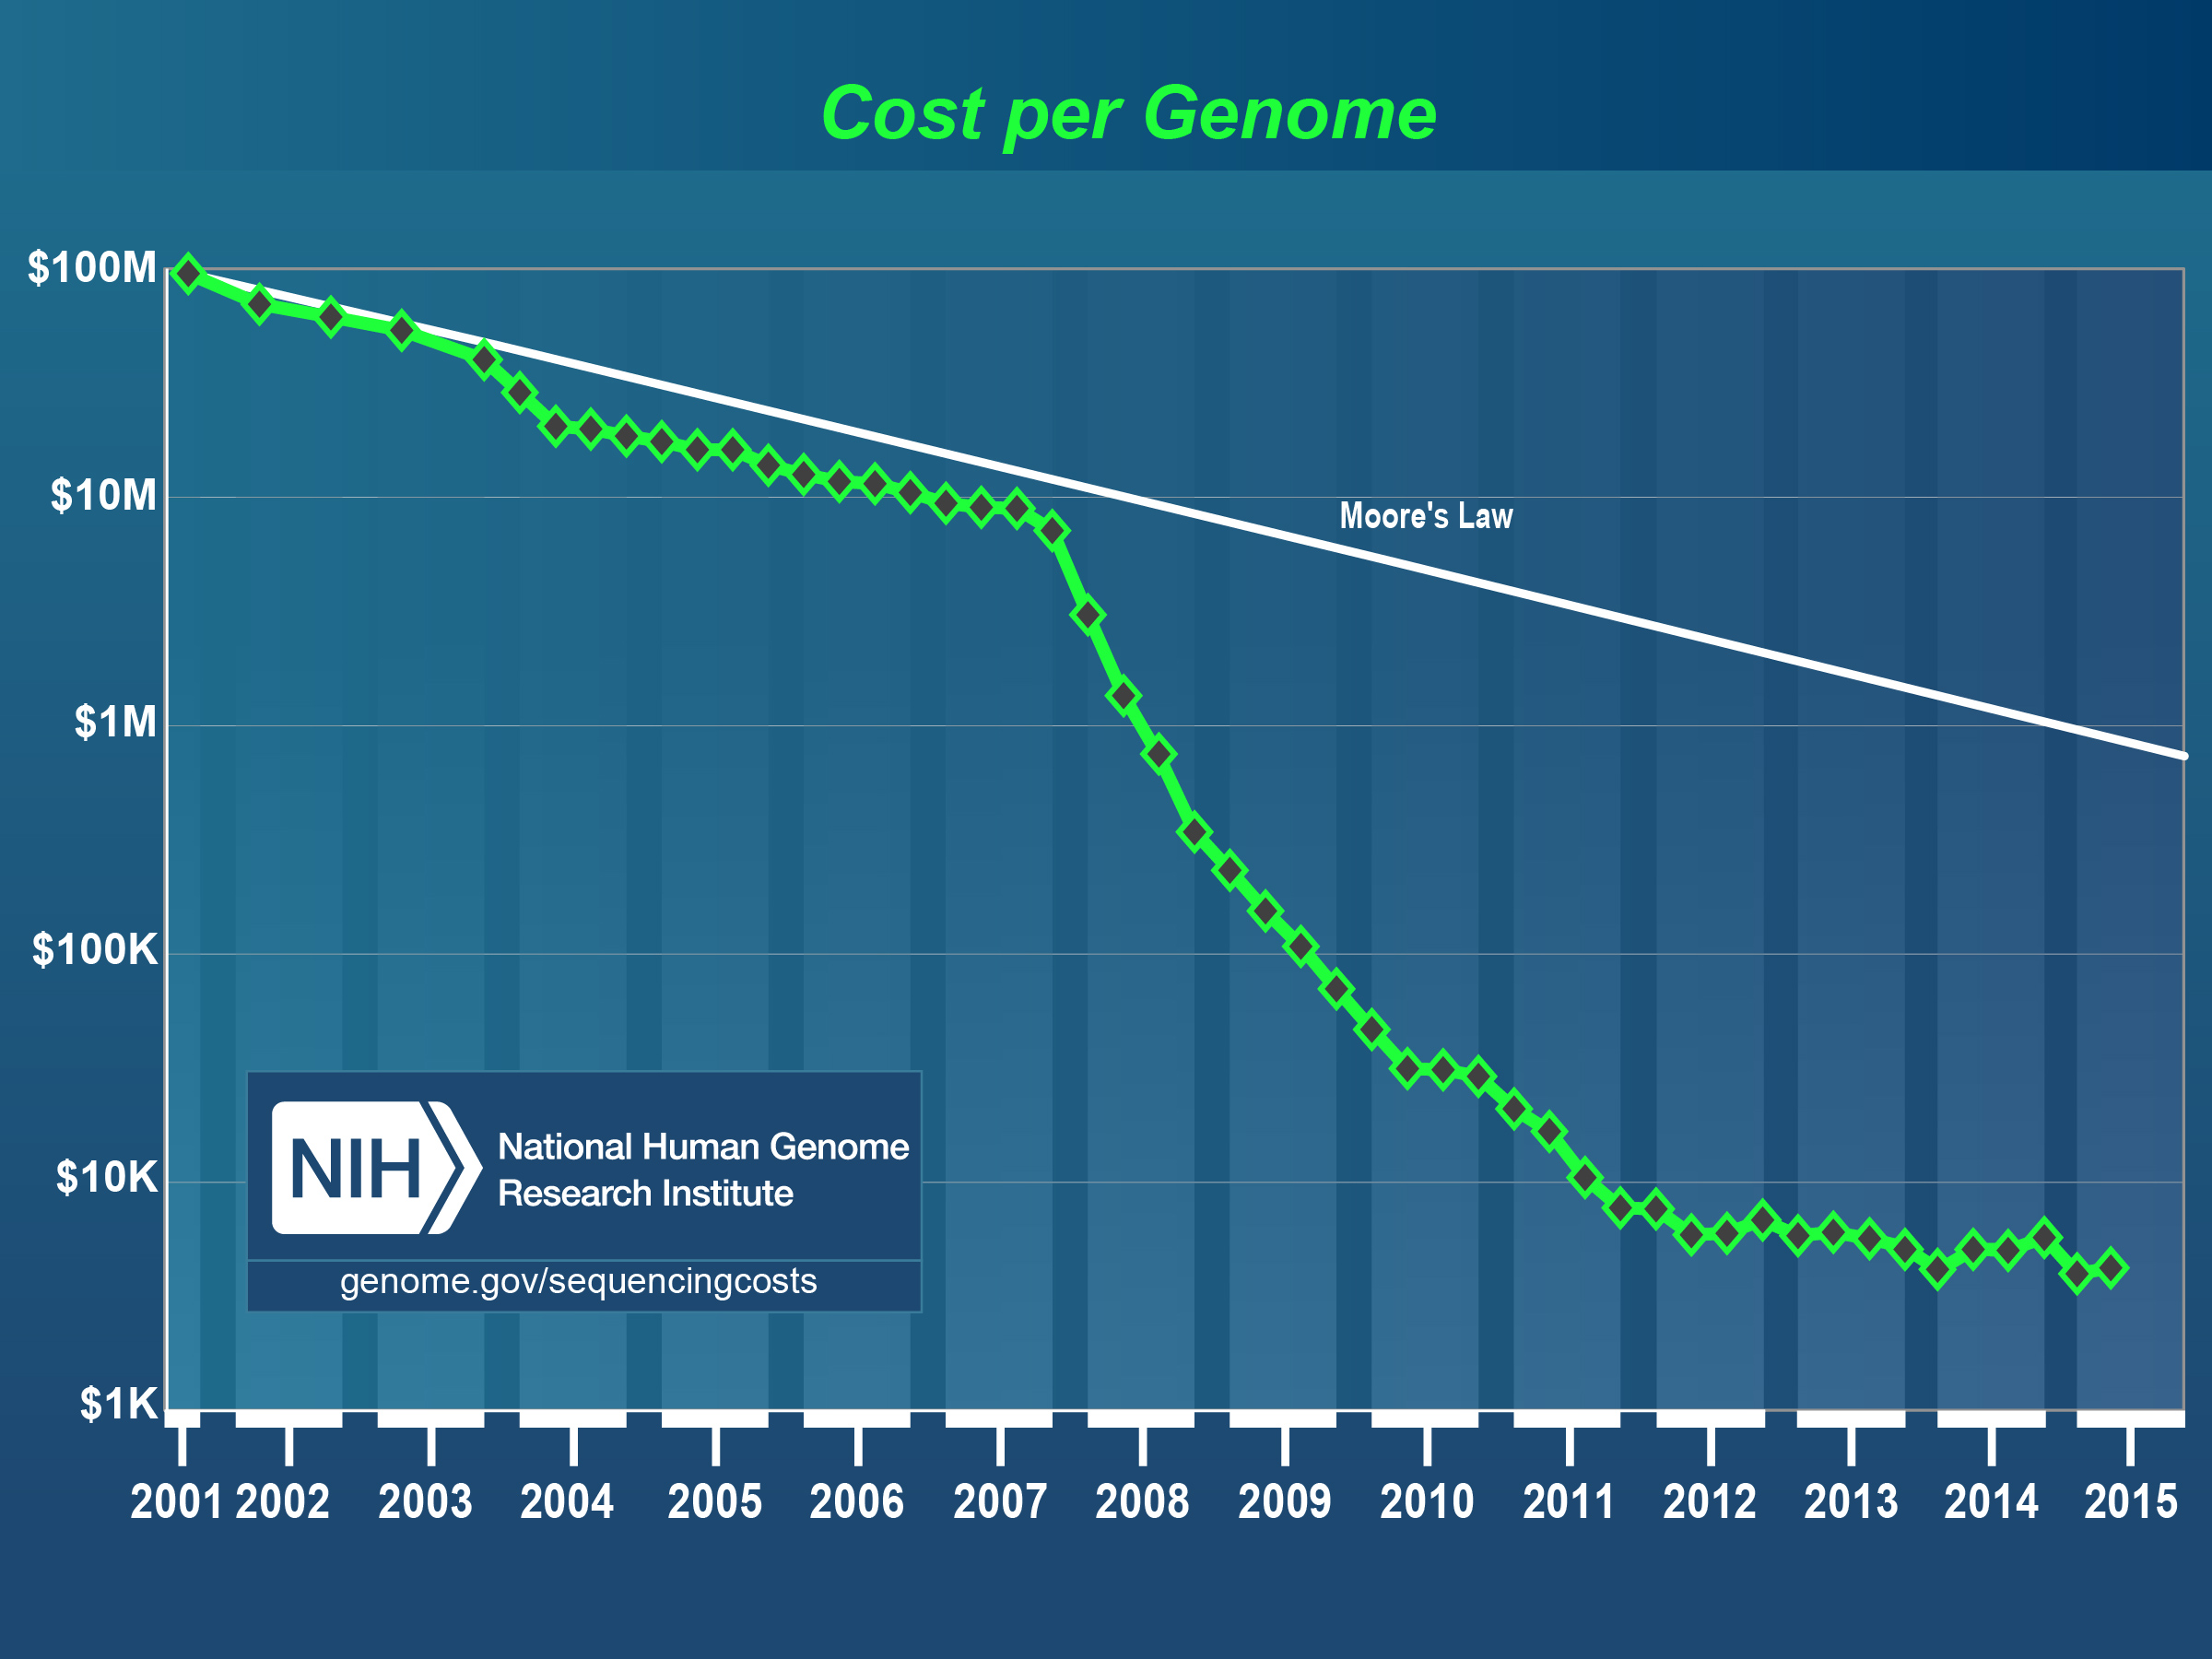
\includegraphics[width=0.5\linewidth]{figures/costpergenome_apr2015.jpg}}
\caption{\label{fig:costs}Trend der Genomesequenzierungskosten (NHGRI). Neben den Kosten zeigt die Grafik das sogenannte Mooresche Gesetz. Es beschreibt den langzeit Trend in der Computer Hardware Industrie. Die plötzlich einsetzende Entfernung der sinkenden Kosten vom Mooreschen Gestz im Jahr 2007 wird mit dem Übergang von Sanger-bastierten Sequenzierung zu 'second generation' oder 'next-generation'-Technologien erklärt \cite{sequencingCosts}.}
\end{figure}

Zwar sinken ebenfalls die Kosten für die Speicherung, allerdings ist der Fortschritt in der Sequenzierungstechnologie dem der Hardware Industrie weit voraus \cite{sequencingCosts}.  Das Resultat sind immer größere Mengen an produzierten Daten. Sie stellen nicht nur für die langfristige und sichere Speicherung eine Herausforderung dar, sondern auch für deren Prozessierung und Analyse. Je größer die Daten desto höher sind die Anforderungen an die Ausstattung des benutzten Computers. Oft kann dadurch nur mit sehr hochwertigen, kostspieligen \textit{'high-end'} Computern gearbeitet werden. Wer keinen besitzt, muss oft auf externen Servern arbeiten, was wiederum zu einem zeitaufwändigen Datenransfer führt.
Um diesen Problemen entgegenzuwirken, ist ein vielversprechender Lösungsansatz die Kompression der Daten. Da Sequenzdaten generell textbasiert gespeichert werden, finden die Grundlagen der Kompression von Texten Anwendung. \\

Ziel der Kompression ist es, eine Datei in einer Art und weise zu Verändern, bzw. zu Kodieren, sodass die dabei entstehende Version weniger Speicherplatz (Byte) als vorher benötigt. Ist die Kompression verlustfrei, kann die Originaldatei ohne Informationsverlust wieder vollständig dekodiert werden. Falls kleine, statisch nicht signifikante Unterschiede toleriert werden können, werden in manchen Fällen verlustreiche Methoden der Kompression aufgrund der Effizienz bevorzugt. Da bei DNS-Sequenzen schon kleinste Unterschiede von großer Bedeutung sein können (z.B. Single Nucleid Polymorphism (SNP)), wird eine verlustreiche Kompression vermieden und soll in dieser Arbeit nicht weiter thematisiert werden. Grundsätzlich unterscheidet man zwischen bit-manipulierender, statistischer und Wörterbuch-basierter Kompression.

Die Idee der Bit-Manipulation ist es zwei oder mehr Zeichen als mit Hilfe von Bit-Kodierung in einem einzigen Byte zu speichern. Durch verschiedene Kombinationen und limitierte Alphabete können so Kompressionsraten von 1:4 erreicht werden \cite{rani14new}. Statistische Methoden entwickeln Modelle, welche das nächste Zeichen voraussagen oder die abgeleiteten Häufigkeiten für eine sinnvolle Kodierung verwenden. Wörterbuch-basierte Methoden hingegen benutzen Substitution, um wiederholt auftretende Teilsequenzen durch einen Zeiger auf einen entsprechenden Wörterbucheintrag zu ersetzen. 

Einer der am häufigsten als Basis benutzte Wörterbuch-basierten Algorithmen ist der Lempel-Ziv-Welch-Algorithmus (LZW) \cite{Ziv77auniversal}. Er komprimiert verlustfrei jedes Format, da das dynamisches Wörterbuch erst bei Start des Verfahrens aufgebaut wird. Eine weitere, sehr wichtige Methode, ist die Huffman-Kodierung \cite{huffman}. Sie weist einer festen Anzahl von Symbolen eine Bit-Codierung (Codewort) mit variabler Länge zu. Dabei bekommen häufig auftretende Symbole die kürzesten Codewörter, um so die Eingabe mit optimaler (kleinster) Länge zu kodieren. Oft werden beide Algorithmen kombiniert (\cite{software:gzip}).

Im Zuge der immer größeren Nachfrage nach speicherplatzeffizienten Formaten für DNS, wurde noch eine weitere Art der Kompression entwickelt.

Die \emph{referentielle Kompression} geht auf die spezifischen Eigenschaften von von DNS ein. Ähnlich der Wörterbuch-basierten Variante, werden bei der referentiellen Kompression ebenfalls Zeiger verwendet. Sie verweisen allerdings auf Teile einer Referenzsequenz anstatt eines Wörterbucheintrags. Man macht sich hierbei die Tatsache zu Nutze, dass, besonders innerhalb einer Spezies, die Ähnlichkeit zwischen Sequenzen sehr hoch ist. Beispielweise unterscheiden sich statistisch gesehen im durchschnitt zwei zufällige Humangenome um nur ca. 0,1$\%$ \cite{Venter16022001}. Folglich kann man 99,9$\%$ der Sequenz als Zeiger auf eine Referenz kodieren und sollte somit eine sehr hohe Kompression erreichen können. Der Nachteil dieses Verfahrens ist die starke Abhängigkeit von der verwendeten Referenz. Vergleicht man ein Humangenom mit z.B. einem Mausgenom würde man nur eine geringe Kompression erreichen können. \cite{wandelt14trends} schätzt die Länge von gleichen Teilsequenzen zwischen Maus und Mensch auf nur ca. 20-25 Basen, wodurch eine Kodierung ähnlich der Grafik~\ref{fig:refKomp}, mehr Speicherplatz als vorher verbrauchen würde. Folglich ist die referentielle Kompression weitestgehend für sogenannte Resequenzierungs-Projekte (\textit{resequencing}) geeignet, welche sich auf die Sequenzierung von Genomen innerhalb einer Spezies konzentrieren. \\

\begin{figure}
\centering{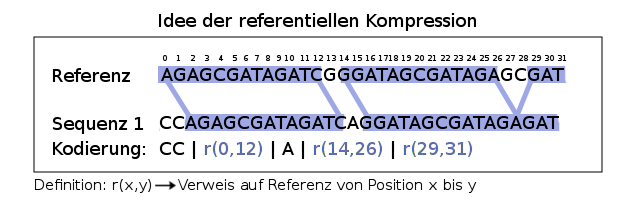
\includegraphics[width=0.8\linewidth]{figures/referentielle_kompression.png}}
\caption{\label{fig:refKomp}Idee der referentiellen Kompression. }
\end{figure}

Es existieren bereits einige Algorithmen und Programme mit verschiedenen Ansätzen für die referentiellen Kompression von DNS. Methoden die auf die Kompression von Rohdaten in Form von \textit{reads} abzielen (\cite{deorowicz11fastq}) werden vernachlässigt, da sie trotz ähnlicher Problemstellung nur sehr gering auf das Ziel dieser Arbeit übertragbar sind. Der Fokus liegt auf Algorithmen für die Kompression von ganzen Genomen bzw. Genomsammlungen.
Erste erfolgreiche Resultate konnten 2008 von \cite{christley09email} verzeichnet werden: Das James Watson Genom wurde von ~3.1 GB auf lediglich ~4.1 MB komprimiert. Allerdings wurde hierbei das Wissen von genauen Unterschieden, namentlich SNP's und kurze Indel's, zum Referenzgenom vorausgesetzt. Das heißt, die Eingabe für den Algorithmus ist das durch \textit{Variant Calling} vorprozessierte VCF-Format (\textit{Varaint Calling Format}). Ebenfalls auf VCF-Basis erzielte \cite{deorowicz13TDC} die bisher höchste höchste Kompressionsrate von ca 1:15000, auf den Daten des \textit{1000 Genome Projects}.

Das Problem des Variant Calling ist jedoch äußerst schwierig, denn es erfordert ein perfektes globales Alignment zum entsprechenden Referenzgenom. Häufig kann diese nötige Voraussetzung  nicht erfüllt werden. Aus diesem Grund muss zu den Algorithmen, welche auf reinen Sequenzdaten (FASTA-Format oder ähnliches) arbeiten können, unterschieden werden. Eine Übersicht dieser Algorithmen bis 2013 wird in dem Bericht \cite{deorowicz13info} aufgestellt (Grafik 3 – gekürzte Originaltabelle).

\begin{figure}
\centering{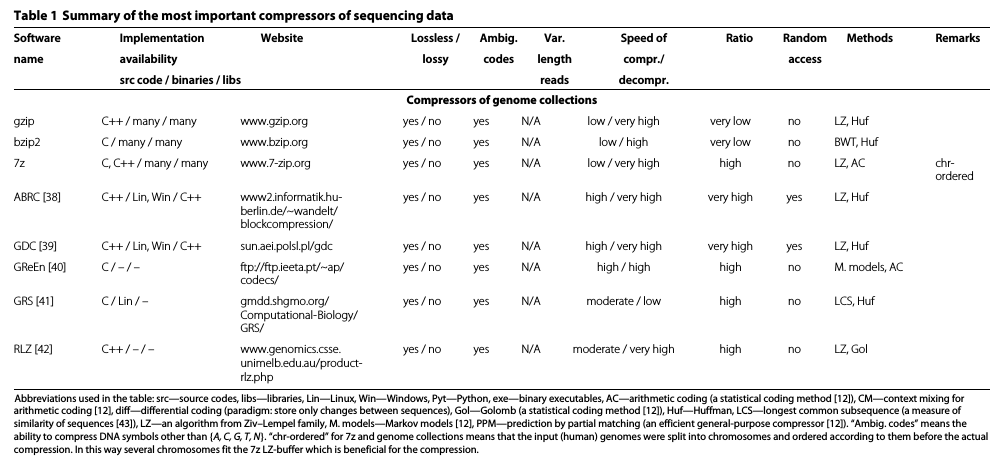
\includegraphics[width=1\linewidth]{figures/tabelle_sequence_compressors.png}}
\caption{\label{fig:seqComp} Zusammenfassung der wichtigsten Kompressoren von Sequenzdaten}
\end{figure}

Die Programme gzip, bzip2 und 7z (Referenzen notwendig?), sind allgmeine, textbasierte Kompressoren, deren Kompression, unter Ausnahme von 7z, sehr gering eingeschätzt wird. Tatsächlich erzielt das sehr verbreitete Programm gzip lediglich eine Rate von ca. 1:4 (???nachgucken referenz).
Dagegen erzielen die speziell für genomische DNS entworfenen Programme deutlich bessere Ergebnisse. Die zwei Algorithmen GRS~\cite{wang11GRS} und GreEn~\cite{pinho12Green} verzeichnen Kompressionsraten für einzelne Humangenome von ca. 1:200. Während GRS als Basis das Prinzip der \textit{Longest Common Subsequence} mit anschließender Huffman-Codierung benutzt, verwendet GreEn einen statischen Ansatz mit Hilfe Markov-Modellen. Ein Ansatz mittels der Lempel-Ziv Methode LZ77 wird von \cite{Kuruppu:RLZ} vorgeschlagen (RLZ) und erreicht ähnliche Kompressionraten von 1:250. Ein weiterer Kompressionsalgorithmus (ABRC) wurde von Wandelt und Leser angeboten, der einen komprimierten Suffixbaum für die Suche von Gemeinsamkeiten blockweise aufbaut \cite{wandelt:ABRC}. Durch anschließende Lempel-Ziv Transformation und Huffman-Kodierung erreicht das Programm ABRC Kompressionsraten von 1:400 auf Daten des \textit{1000 Genome Projects}. Eine noch höhere Kopressionsrate erreichte der Algorithmus GDC (Rate ca. 1:600) bzw. GDC Ultra (Rate ca. 1:2000) \cite{deoriwicz:GDC}, gefolgt von GDC 2 (Rate ca. 1:9000) \cite{deoriwicz:GDC2}. Ähnlich dem Programm RLZ basiert der GDC/GDC-Ultra/GDC 2 Algorithmus auf LZ77,  allerdings mit einem wichtigen Unterschied zu anderen Methoden. Alle vorherigen Methoden komprimieren auch bei einer Sammlung von Genomen jedes einzelne unabhängig. Im Gegensatz dazu, werden bei GDC mehrere Sequenzen als Referenz genutzt. Die zusätzliche Zusammenführung von Informationen zwischen den zu komprimierenden Sequenzen, stellt sich als sehr vielversprechende Idee da.\\

Über die Anstrengungen zur Reduzierung des Speicherplatzes und des Datentransfers hinaus, muss auch die zeitaufwändige Analyse solcher Datenmengen beachtet werden. Alle bisher angesprochenen Algorithmen, dienen lediglich der Kompression von Daten hinsichtlich ihrer Speicherung. Will man die Daten analysieren, müssen sie wieder dekodiert werden. Die Sequenzen bzw. Genome würden zudem einzeln und nacheinander untersucht werden. Man verwirft dabei die vorher zur Kompression benutzte Information der hohen Ähnlichkeit zwischen Sequenzen, was zur überflüssigen Analyse von redundanten Teilsequenzen führt. Es liegt folglich nahe, die referentielle Kompression auch auf die Analyse zu erweitern. Diese Problemstellung wird von \cite{loh12compressivegenomics} als \textit{compressive genomics} benannt. 

Die erste Möglichkeit, verschiedene sequentielle Algorithmen auf mehreren Sequenzen gleichzeitig laufen zu lassen, wird von \cite{Rahn15072014} vorgestellt. Durch eine unterliegende Datenstruktur, als JST (\textit{journaled string tree}) bezeichnet, werden Sequenzen als eine Menge von Varianten, basierend auf einem gemeinsamen Koordinatensystem repräsentiert. Eine einzelne Sequenz kann wiederum aus ihren zugehörigen Varianten, als referentiell komprimierter String (\textit{journaled string}), generiert werden. Durch die referentielle Kompression von Sequenzen zu Varianten, werden gemeinsame Bereiche nur einmal analysiert und die Laufzeit wird um den Faktor 115 Beschleunigt \cite{Rahn15072014}.

\subsection{Motivation}
Die Arbeit beschäftigt sich mit der Implementierung eines C++ Programms innerhalb der SeqAn Bibliothek \cite{doering08seqan}, welches der verlustfreien referentiellen Kompression von DNS-Sequenzen dienen soll. Sie steht in engem Zusammenhang mit dem SeqAn Projekt des JST \cite{Rahn15072014} und ist auf dessen Kompatibilität abgestimmt.

Derzeit können zur Verwendung des JST nur Dateien im VCF-Format benutzt werden. Das Hauptinteresse liegt daher nicht nur in der bestmöglichen Speicherplatzreduzierung einer Datei, sondern in der möglichst effizienten Transformation und Speicherung der Eingabedaten (FASTA-Format o.ä.) in einem für den JST weiterverwendbares Format. 

Der vorgestellte Algorithmus soll lediglich die Unterschiede zur Referenz kodieren und dabei die Idee der Zusammenführung von Informationen zwischen den zu komprimierenden Sequenzen von \cite{deoriwicz:GDC,deoriwicz:GDC2} aufgreifen. Da viele Autoren auf die Abhängigkeit der Kompression von der verwendeten Referenzsequenz hindeuten \cite{deorowicz13info,wandelt14trends,kuruppu:refseq}, ist eine Besonderheit gegenüber anderen Arbeiten, dass die verwendete Referenzsequenz variabel sein soll. Sie wird bei jeder Eingabe neu angelegt und kann fortlaufend verändert werden, mit dem Ziel, das Speicherformat weiter zu optimieren.

%%%%%%%%% METHODen %%%%%%%%%%%%%%%%%%%%%%%%%%%%%%%%%%%%%%%%%%%%%%%%%%%%%%%%%%%%%%
\section{Methoden}

\subsection{Definitionen und allgemeine Notation}
\label{sec:definitions}
Ein \textbf{String} \textit{s} $=$ $s_{0}$....$s_{n-1}$, $ s_{i} \in \sum$, ist eine Sequenz der Länge $|s| = n$, auf Basis des Alphabets $\sum$. Ein Teilstring von \textit{s}, von Position \textit{i} bis \textit{j}, wird als \textit{s}[\textit{i},\textit{j}] = $s_{i}$....$s_{j-1}$ angegeben. Falls $i\ge j$, wird die Rückgabe als leerer String definiert. Der Spezialfall \textit{s}[\textit{i}, \textit{i+1}] wird zu \textit{s}[\textit{i}] abgekürzt.  \\

Ein \textbf{Journaled String} verhält ich wie ein normaler \textit{String} (Notation s.o.), mit dem Unterschied, dass er aus zwei Datenstrukturen besteht. Die Erste, der \textit{'Holder'}, speichert die Referenzsequenz. Die Zweite speichert Veränderungen mittels eines \textit{journal tree} und eines \textit{insertion buffers} [referenz rene].\\

Ein \textbf{Journal Entry} ist ein Eintrag im \textit{journal tree} eines \textit{journaled string} der eine Veränderung der Referenzsequenz beschreibt. Für mehr Details siehe [referenz rene].\\

Ein \textbf{Seed} ist ein Tupel $seed=$($b_{r},b_{s},e_{r},e_{s}$) und beschreibt einen gemeinsamen Teilstring von zwei Strings $r$ und $s$. Es gilt: $r$[$b_{r},e_{r}$] $=$ $s$[$b_{s},e_{s}$]. Die Länge $|seed|$ wird definiert als $b_{r}-e_{r} = b_{s}-e_{s}$ .\\

Ein \textbf{Repeat} ist ein sich wiederholender Teilabschnitt innerhalb einer Sequenz. Formal wird er hier folgend definiert: \textit{Seed} $a = (b_{1r},b_{1s},e_{1r},e_{1s})$ und \textit{seed} $b=(b_{2r},b_{2s},e_{2r},e_{2s})$, welche beim untersuchen eines q-grams von $s$ gegen die Referenz $r$ gefunden werden, beschreiben dann einen Repeat, wenn $|b_{1r} - b_{2r}| < q $. \\

Ein \textbf{$\Delta$-Event} $e = (pos,type,seqs,ins,del)$ repräsentiert eine Veränderung einer Referenzsequenz $r$ and der Position \textit{pos}. Es kann einen von vier Typen annehmen (\textit{type}): SNP, Deletion(DEL), Insertion(INS) und strukturelle Variation(SV). Mit Hilfe von \textit{seqs} wird gespeichert, in welchen Sequenzen e vorkommt. \textit{ins} bezeichnet einen String der an Stelle \textit{pos} eingefügt wird und \textit{del} die Länge des Teilstrings $r[pos,pos+del]$ der gelöscht wird.\\

Eine \textbf{dependent region} ist eine Gruppe von $\Delta$-Events, welche jeweils direkt oder indirekt voneinander abhängig sind. Definition von Abhängigkeit: $e_{1} = (pos_{1},type_{1},seq_{1},ins_{1},del_{1})$, $e_{2} = (pos_{2},type_{2},seq_{2},ins_{2},del_{2})$, o.B.d.A gilt $pos_{1} \le pos_{2} $; dann ist $e_{1}$ ist direkt abhängig von $e_{2}$  $(e_{1}\sim e_{2})$ wenn: $(pos_{1}+del) > pos_{2} $. $e_{1}$ ist indirekt abhängig von $e_{2}$,  wenn ein Event (oder eine Kette mehrerer Events) $e_{i}$ existieren, sodass gilt $(e_{1}\sim e_{i} \wedge e_{i}\sim e_{2})$.

%


\subsection{Konzept}

\begin{figure}
\centering{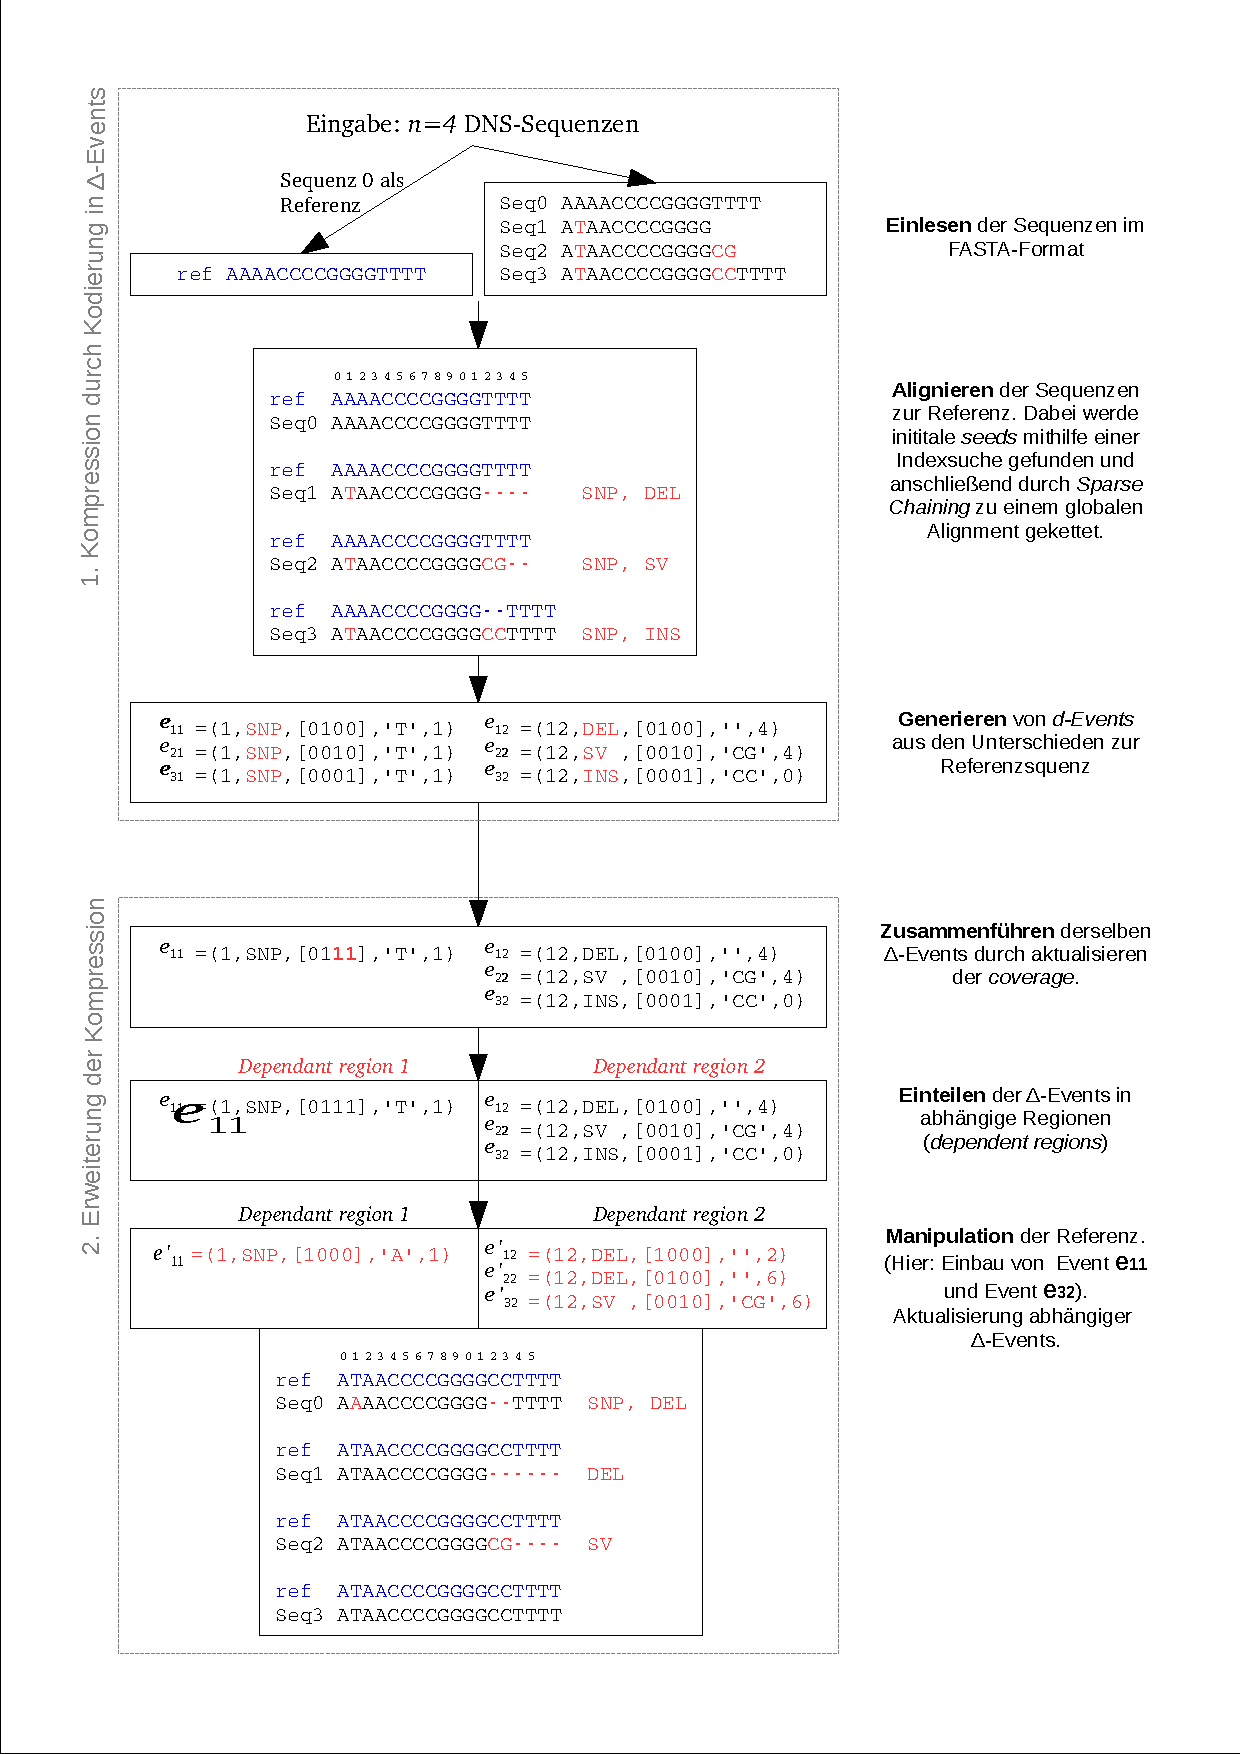
\includegraphics[width=0.9\linewidth]{figures/konzept.pdf}}
\label{fig:konzept}
\caption{Konzept des Kompressionsalgorithmus' anhand eines Beispiels.}
\end{figure}

Der vorgestellte Algorithmus kann grundlegend in in zwei Abschnitte unterteilt werden: Dem "Variant Calling" und der Verbesserung der Kompression durch Evenprozessierung. Die Eingabe erfordert Sequenzen im FASTA-Format, welche komprimiert in die Enddatenstruktur, die DeltaMap, überführt werden. Zur Visualisierung ist ein Beispiel in Grafik~\ref{fig:konzept} dargelegt.

Beim \emph{"Variant Calling"} (Sektion~\ref{sec:varcall}) werden Sequenzen gegen eine Referenz aligniert, um die daraus resultierenden Unterschiede zur Referenz als $\Delta$-Events abzuspeichern. Diese Methode entspricht vom Prinzip her dem \textit{Variant Calling} zur Erstellung eines VCF-Formats (GATK~\cite{GATK:variantcalling}). Der Unterschied ist, dass kein perfektes globales Alignment erstellt wird und die $\Delta$-Events somit nicht mit den VCF-Einträgen vergleichbar wären.
Zunächst werden hierzu die Sequenzen eingelesen und die erste dient im Folgenden als Referenz. Durch eine Index-basierte Suche werden \textit{seeds} zwischen den einzelnen Sequenzen und der Referenz gefunden und erweitert. Die Menge an gefundenen \textit{seeds} wird anschließend zu einer globalen Kette reduziert. Die globale Kette kann als Repräsentation eines Alignments gesehen werden. Die Bereiche zwischen den gewählten \textit{seeds} der globalen Kette stellen die Unterschiede, oder auch Varianten, dar und werden als $\Delta$-Events gespeichert.

Die \emph{Eventproessierung} (Sektion~\ref{sec:evepro}) soll die Anzahl der generierten $\Delta$-Events, sowie den Speicheraufwand der Enddatenstruktur (DeltMap) verringern. Hierzu werden als Erstes gleiche Events auf verschiedenen Sequenzen als ein Event zusammengeführt. Die Kodierund der Sequenzen in Events entspricht nun eher einem Multilen-Alignment. Nachfolend werden voneinander abhängige Events zur weiteren Evaluierung in Gruppen eingeteilt (\textit{dependent regions}). In Jeder Gruppe wird den jeweiligen Events dann ein Score zugewiesen, welcher die mögliche Speicherverringerung beschreibt. Je nach Score werden einige Events in die Referenzsequenz eingebaut und die Sequenzkodierung wird entsprechend aktualisiert. 

\subsection{Implementierung - "Variant Calling"}
\label{sec:varcall}

\subsubsection{Indexsuche}
Die Suche nach Gemeinsamkeiten zwischen einer Sequenz und ihrer Referenz ist eines der Schlüsselprobleme bei der referentiellen Kompression. In dem hier vorgestellten Algorithmus wird dazu zunächst ein q-Gram-Index über der Referenz aufgebaut. Die Wahl des Parameters q wird dem Benutzer überlassen. Allerdings wird empfohlen, das q bei genomischer DNS über 15 liegen sollte, damit zufällige q-mere vermieden werden \cite{wandelt14trends}. Da bei großen Werten für q, auf einem Alphabet $\sum$, die Anzahl an möglichen q-meren exponentiell steigt ($|\sum|^{q}$), wird ab einem Wert von 
\begin{equation}
q>log_{|\sum|}(RAM~Speicher~in~Byte)
\end{equation}
das \textit{OpenAdressing()} (SeqAn \cite{doering08seqan}) verwendet. Beim \textit{OprenAdressing()} werden nur solche q-mere gespeichert, die auch tatsächlich in der indizierten Sequenz zu finden sind.

Wird jede der $m$ Eingabesequenzen, mit einer jeweiligen Durchschnittslänge $n$, sequentiell nach gemeinsamen q-meren durchsucht, ergibt sich trotz Zugriff auf den q-Gram-Index in $O(1)$ eine Laufzeit von $O(n*m)$. Aus diesem Grund wird die Suche um einige Faktoren erweitert, die auf die spezifischen Eigenschaften von DNS eingehen.

\subsubsection{Verbesserung der Suche}
Die Indexsuche wird um folgende vier Punkte erweitert:

(1) \emph{Ignorieren von Repeats}. Genomische DNS enthält meist sehr viele repititive Abschnitte. Umfasst ein q-gram einen Repeat würde er die Suche enorm verlangsamen, denn pro q-gram in der durchsuchten Sequenz würden viele tausende in der Referenz gefunden werden. Solche q-gramme werden als Treffer ignoriert, indem jeder gefundene seed mittels seines Vorgängers auf einen Repeat getestet wird (siehe formale Definition in Sektion~\ref{sec:definitions}). Ähnlich verhält es sich auch, falls das DNS-Alphabet um den Buchstaben 'N' erweitert ist und ein q-gram ausschließlich aus 'N' besteht. Sie werden ebenfalls ignoriert.

\begin{figure}[b]
\centering{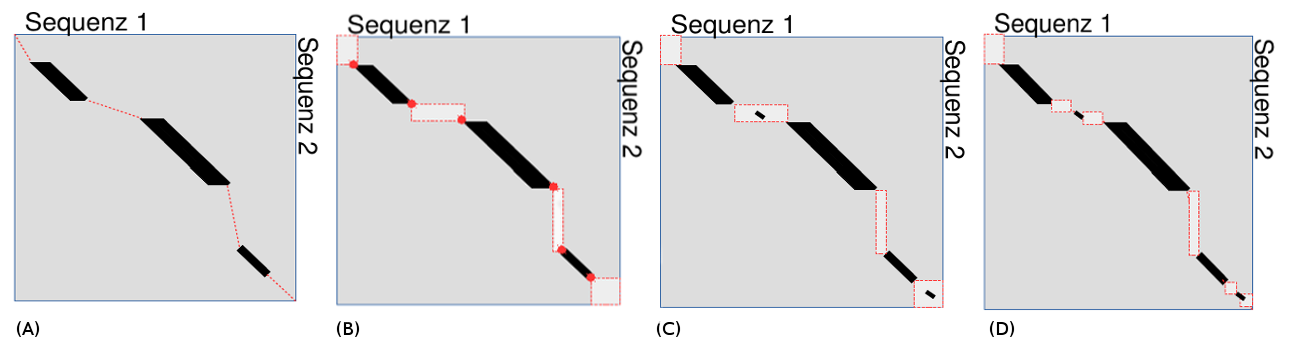
\includegraphics[width=0.9\linewidth]{figures/iterativer_schritt.png}}
\label{fig:iterativ}
\caption{Iterative Schritte in der Indexsuche. In (A) sind in der initialen Suche drei große \textit{seeds} gefunden und für die globale Kette selektiert worden. Wie in (B) dargestellt, ergeben sich dadurch Bereiche zwischen den \textit{seeds}; Jeweils von der rechten unteren Ecke des vorhergehenden \textit{seeds} zu linken oberen Ecke des darauffolgenden. In (C) sind dadurch kleinere \textit{seeds} gefunden worden, die zu neuen Bereichen wie in (D) führen.}
\end{figure}

(2) \emph{Iterativer Schritt}(Grafik~\ref{fig:iterativ}). Die Schnelligkeit kann auf kostet der Sensitivität erhöht werden, wenn der Benutzer einen relativ hohen Wert für $q$ wählt. Um dennoch eine ausreichende Genauigkeit zu gewährleisten, können im Programmaufruf ein oder mehrere iterative Schritte mit niedrigeren Werten für $q$ spezifiziert werden. Der Algorithmus durchläuft dann eine initiale Suche mit dem ersten $q$-Wert, speichert die resultierende globale Kette und starten dann in den Bereichen zwischen den ausgewählten \textit{seeds} der Kette einen erneute Suche mit dem nächsten Wert für $q$. Diese Methode ist der des LAGAN Algorithmus für globale Alignments nachempfunden \cite{brudno03lagan}.

(3) \emph{Initiale Suche mit dynamischen Offset}. Diese Erweiterung basiert auf der Erwartung, dass bei sehr ähnlichen Sequenzen lange gleiche Abschnitte zwischen einer Sequenz und ihrer Referenz existieren. Anstatt eine sequentielle Suche (Offset=1 oder q) durchzuführen, wird in jedem Schritt der Suche ein neuer Offset bestimmt.  Hierfür wird an einer Position $p$ in der Sequenz jeder gefundene $seed_{i}(p)$ (jedes initiale q-gram) zunächst erweitert. Die Erweiterung, bzw. Verlängerung des \textit{seeds}, erfolgt solange in beide Richtungen, bis ein \textit{mismatch} (Unterschied) auftritt. Anschließend wird jedem Seed ein Score 
\begin{equation}
Score(seed)=|seed_{i}(p)|+diagonal(seed_{i}(p))
\end{equation}
zugewiesen, wobei $diagonal(seed_{i}(p))$ die Abweichung zur Hauptdiagonalen angibt. Die Länge des \textit{seeds} mit dem besten 
Score wird als neuer Offset gesetzt und die Suche auf der Sequenz wird an Position $p+offset$ fortgeführt. Etwaige Verluste an Sensitivität können durch iterative Schritte wieder ausgeglichen werden.

(4) \emph{Parallelisierung der initialen Suche}. Um die Suche abermals zu beschleunigen wird die initiale Suche parallelisiert. In Anlehnung an \cite{rani14new}, wird die zu untersuchende Sequenz in Blöcke aufgeteilt. Jeder Block wird einzeln nach Gemeinsamkeiten untersucht aber im Gegensatz zu \cite{rani14new}, werden die Blöcke vor der weiteren Analyse (und Kodierung) wieder zusammengeführt. Somit entsteht kein Informationsverlust und die Ergebnisse entsprechen denen ohne Parallelisierung.

\subsubsection{Reduktion zu einer globalen Kette}
Für die Reduktion einer Menge von \textit{seeds} wird der \textit{Sparse Chaining} Algorithmus von \cite{gusfield97algorithms} verwendet. Er konstruiert in $O(r*log(r))$ eine optimale globale Kette von \textit{seeds}, denen ein bestimmtes Gewicht (Score) zugewiesen wurde. Der Algorithmus ist bereits in der SeqAn-Bibliothek \cite{doering08seqan} enthalten und benutzt dort als Gewichtung die Länge des \textit{seeds}. Die Gewichtung ist geeignet, da längere Gemeinsamkeiten später eine geringere Anzahl an $\Delta$-Events bedeuten und somit zu bevorzugen sind.

Um die Laufzeit des Programmes zu verbessern, ist dem Benutzer möglich für den initialen Suchlauf (und nur für diesen) eine Mindestlänge der \textit{seeds} zu spezifizieren. Liegt ein gefundener \textit{seed} bei der Suche unterhalb dieser Länge wird er wieder verworfen. Mit dieser Einschränkung lässt sich die Anzahl an \textit{seeds} kontrollieren, um den \textit{Chaining}-Algorithmus zu entlasten. Auch hier wird ein drohender Verlust an Sensitivität, durch ausscheiden einiger mitunter wichtigen \textit{seeds}, mit Hilfe des iterativen Schritts ausgeglichen.

\subsubsection{Generierung von $\Delta$-Events}

\begin{figure}[t]
\centering{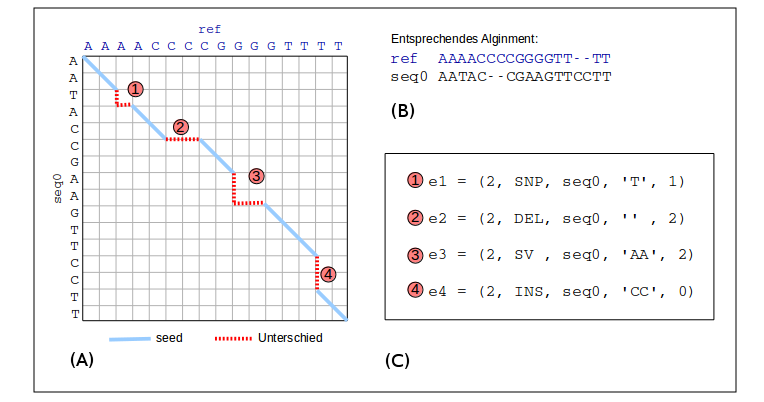
\includegraphics[width=0.9\linewidth]{figures/delta_events.png}}
\caption{\label{fig:deltaevent}\emph{Generierung von $\Delta$-Events}. Abbildung (A) visualisiert das Ergebnis der Indexsuche. Die Bereiche zwischen den \textit{seeds} bilden die Vorlage für die $\Delta$-Events. (B) zeigt die entsprechende Alignment-Repräsentation und (C) die generierten $\Delta$-Events.  }
\end{figure}

Steht die globale Kette fest, repräsentiert sie ein globales Alignment zwischen der untersuchten Sequenz und der Referenz. Jeder \textit{seed} beschreibt dabei eine gemeinsame Teilsequenz, wohingegen die Bereiche dazwischen Unterschiede bzw. Varianten darstellen. Jeder dieser Zwischenbereiche wird zu einem einzelnen $\Delta$-Event, indem die zwei angrenzenden \textit{seeds} mittels Manhattan-Distanz verbunden werden. Die Position eines $\Delta$-Events wird dabei als absolute Position in der Referenz gespeichert (Abbildung~\ref{fig:deltaevent}).

\emph{Formale Definition}. \textit{Seed} $a = (b_{1r},b_{1s},e_{1r},e_{1s})$ und \textit{seed} $b=(b_{2r},b_{2s},e_{2r},e_{2s})$ liegen hintereinander in der globalen Kette, welche durch Analyse der i-ten Sequenz $s$ gegen die Referenz $r$ erstellt wurde. O.B.d.A liegt $a$ über und links von $b$. Dann werden aus dem Bereich zwischen $a$ und $b$ folgende Attribute für das Event $e$ definiert:
\begin{equation}
pos_{e} = e_{1r}
\end{equation}
\begin{equation}
ins_{e} = s[e_{1s},b_{2s}]
\end{equation}
\begin{equation}
del_{e} = b_{2r}-e_{1r}
\end{equation}
\begin{equation}
type_{e} = 
\begin{cases}
SNP & falls~ |ins| = 1~ und~ del = 1, \\
DEL & falls~ |ins| = 0, \\
INS & falls~ del = 0, \\
SV  & sonst
\end{cases}
\end{equation}
$seqs_{e}$ ist ein Bitvektor bestehend aus Nullen, bei dem Position i auf 1 gesetzt wird. Aus diesen Attributen wird anschließend das $\Delta$-Event $e$ generiert:
\begin{equation}
e = (pos_{e}, type_{e}, seqs_{e}, ins_{e}, del_{e})
\end{equation}

\subsection{Implementierung - Verbesserung der Kompression}
\label{sec:evepro}
Die Darstellung der Eingabesequenzen als $\Delta$-Events kann bereits als referentielle Kompression gesehen und als solche verwendet werden. Nichtsdestotrotz soll die Kompression weiterhin verbessert werden. Hierzu werden zwei Ansätze verfolgt: 

Vorerst sollen gleiche $\Delta$-Events auf unterschiedlichen Sequenzen zusammengeführt und gruppiert werden. Dies verringert den Speicherverbrauch. Zum Einen im Arbeitsspeicher für die folgende Prozessierung und zum anderen den Speicherplatz, falls die Events gespeichert werden sollten.

Ziel des zweiten Ansatzes ist die Kompression auf Ebene der \textit{Journaled Strings}. Nach einer Gewichtung (Scoring) der zusammengefassten Events werden manche prozessiert. Mit Prozessierung ist in diesem Fall der eventuelle Einbau eines Events in die Referenz gemeint. Ziel dessen ist es, die Referenzsequenz so zu verändern, dass eine Verringerung der Anzahl an \textit{Journal Entries} erreicht wird.

\subsubsection{Zusammenführung von Events}
Alle gesammelten $\Delta$-Events (aller Sequenzen) werden zu Beginn sortiert. Eine Sortierung erfolgt nach Position, Typ und den Werten für \textit{del} und \textit{ins} in eben gegebener Reihenfolge. Nun wird die aufsteigend sortierte Liste durchlaufen. 

Gleiche Events sollten durch die Sortierung hintereinander liegen und nun können durch Aktualisierung des \textit{seqs}-Vektors zusammengeführt werden. Der \textit{seqs}-Vektors ist ein Bitvektor mit einer Länge, die gleich der Anzahl an zu komprimierenden Sequenzen ist. Der i-te Eintrag in \textit{seqs} eines Events $e$ gibt an ob $e$ in Sequqnz i vorkommt. Der Bitvektor gewährleistet eine effiziente Speicherung und eine einfache Handhabung mittels logischer Operationen.

\subsubsection{Präprozessierung}
Während der Zusammenführung werden die Events gleichzeitig in Gruppen eingeteilt. Die Gruppen beschreiben voneinander direkt oder indirekt abhängige Events (siehe Sektion~\ref{sec:definitions} für die Definition von Abhängigkeit) innerhalb einer Region der Referenzsequenz (\textit{dependant region}). 
Die Zuteilung der Events in eine Gruppe erfolgt direkt beim Durchlaufen der Liste: Gegeben sei $\Delta$-Event $e_{j}$ in einer aufsteigend sortierte List von Events. Ist $e_{j}$ abhängig von $e_{j-1}$, wird $e_{j}$ derselben Gruppe wie $e_{j-1}$ hinzugefügt. Andernfalls ist die Gruppe von $e_{j-1}$ vollständig und es wird eine neue Gruppe mit $e_{j}$ als erstem Element initialisiert. 

Die Einteilung in Gruppen ist für die nachfolgende Prozessierung von großer Bedeutung. Falls ein Event $e$ durch seinen Einbau in die Referenz deren Sequenzabfolge verändert, sind die von $e$ abhängigen Events davon betroffen und müssen entsprechend aktualisiert werden. Ansonsten kann keine fehlerfreie Kodierung der Sequenzen garantiert werden.

\subsubsection{Prozessierung}
Die Prozessierung von Events geschieht gruppenweise. Dazu wird zunächst für alle Events einer Gruppe $G$ ein Score berechnet (siehe Sektion~\ref{sec:score}). Wird ein Event $e$ durch seinen Score für geeignet befunden, wird es in die Referenz eingebaut.

Der Einbau in die Referenz bedeutet, das die Änderungen, die $e$ beschreibt, in die Referenzsequenz $r$ übernommen werden. Es wird die Teilsequenz $r[pos_{e},~pos_{e}+del_{e}]$ aus $r$ gelöscht und die Teilsequenz $ins_{e}$ an Position $pos_{e}$ eingefügt. Aufgrund der Änderung der Referenz sind nun die übrigen Kodierungen der Sequenzen falsch und müssen aktualisiert werden. Bei einer Aktualisierung wird zwischen Sequenzen, welche direkt abhängige Events zu $e$ besitzen und denen die unabhängig sind, unterschieden. 

Für die unabhängigen oder nur indirekt abhängigen Sequenzen muss lediglich ein neues Event $\tilde{e}$ erstellt werden. $\tilde{e}$ kann als gegenteiliges Event zu $e$ gesehen werden und wird definiert als:
\begin{equation}
\tilde{e} = (pos_{e},~\neg type_{e})~\neg seqs_{e},~r[pos_{e},~pos_{e}+del_{e}],~|ins_{e}|)
\end{equation}
wobei
\begin{equation}
\neg type_{e} =
\begin{cases}
DEL & falls~ type_{e} = INS, \\
INS & falls~ type_{e} = DEL, \\
type_{e} & sonst
\end{cases}
\end{equation}
\\
Für Sequenzen mit von $e$ abhängigen Events muss jedes Event einzeln aktualisiert werden. Es wird dabei vorausgesetzt, das eine Sequenz an einer Position nur ein Event gleichzeitig haben kann. Das heißt, jede Sequenz hat nur ein von $e$ abhängiges Event und folglich können alle abhängigen Events unabhängig voneinander bearbeitet werden. Gegeben das in die Referenz einzubauende Event $e$ und ein von $e$ abhängiges Event $k_{e}$, dann wird $k_{e}$ wie folgt aktualisiert:

\noindent Falls $pos_{e} \le pos_{k_{e}}$
\begin{equation}
k_{e} = (pos_{k_{e}},~*type,~seqs_{k_{e}},.........)
\end{equation}
Falls $pos_{e} \ge pos_{k_{e}}$
\begin{equation}
k_{e} = (pos_{k_{e}},~*type,~seqs_{k_{e}},.........)
\end{equation}
* wobei jeweils $type$ anschließend wie Gleichung (6) ermittelt wird.\\

\noindent Nach der erfolgreichen Prozessierung wird der Vorgang für die aktualisierten Events der Gruppe wiederholt. Falls kein $\Delta$-Event mehr für vorteilhaft befunden wird, wird mit der nächsten Gruppe fortgefahren.
\subsubsection{Scoring - Konzept der Referenzänderung}
\label{sec:score}
Das Scoring (die Gewichtung) von Events kontrolliert die Prozessierung und wird für jede Gruppe unabhängig untersucht. Der Score soll ausdrücken, ob der Einbau des jeweiligen Events in die Referenz hinsichtlich einer Verbesserung der Kompression von Vorteil wäre.

Eine Verbesserung der Kompression bezieht sich in diesem Fall auf die (Arbeits-) Speicherverringung in der Enddatenstruktur. Die Enddatenstruktur ist eine $\Delta$-Map, die in einen JST (\textit{Journaled String Tree}) umgewandelt werden kann (???).  Bei der Analyse mit Hilfe eines JST werden innerhalb eines Kontextes Journaled Strings aufgebaut. Je weniger Journal Entries ein Journaled String hat, desto schneller die Analyse. Ziel ist es also die Anzahl an Journal Entries zu minimieren. (Absatz ist doof...)

Unter dieser Voraussetzung wird der Score eines $\Delta$-Events wie folgt definiert: Gegeben sei $\Delta$-Event $e$. Dann ist $score(e)$ definiert als  die Anzahl an Journal Entries, welche durch den Einbau von e in die Referenz hinzukommen oder wegfallen würden. Es kommt folglich nur ein negativer Score für das Prozessieren in Betracht, da er eine gewünschte Verringerung der Anzahl an Journal Entries verspricht.

Ein Beispiel: Die \textit{dependant region 1} in der Abbildung~\ref{fig:konzept} enthält nur ein Event. Das Event $e_{11}$ ist ein SNP der auf den Sequenzen 1,2 und 3 zu finden ist aber nicht auf Sequenz 0. Das heißt, die drei erstgenannten Squenzen hätten jeweils zwei extra Journal Entries, insgesamt sechs, als Kodierung, während Sequenz 0 keinen Eintrag benötigt. Würde man den SNP in die Referenz einbauen, würden 6 Einträge wegfallen und zwei (für Sequenz 0) hinzukommen.
\begin{equation}
score(e_{11}) = - (2 + 2 + 2) + 2 = - 4
\end{equation}
Da sich kein weiteres Event in der Gruppe befindet ist dieser Score der beste und zu dem negativ: Das Event wird prozessiert.

\subsubsection{Endddatenstruktur}
Wie angesprochen Delta map bla bla
\pagebreak
%%%%%%%%% RESULTS %%%%%%%%%%%%%%%%%%%%%%%%%%%%%%%%%%%%%%%%%%%%%%%%%%%%%%%%%
\section{Ergebnisse}
Die Auswertung wurde auf einem Server der Freien Universität Berlin durchgeführt. Es wurde ein Linux 3.13.0 System mit .... two Intel\textregistered Core\texttrademark i5-3317U CPU's at 1.70GHz (a total of 2 physical and 2 virtual cores) and 5.8GB of RAM. 

Das Programm wurde auf Realdaten getestet. Der erste Datensatz besteht aus bis zu 200 Versionen des menschlichen Chromosoms 21 erhalten vom \textit{1000 Genome Project}~\cite{1000genomes}. Alle Varianten der 1000 Individuen sind einer VCF-Datei gespeichert und mussten für die Analyse zurück in einzelne FASTA-Dateien überführt werden. Hierfür wurde vcf-subset aus dem Paket vcf-tools benutzt, um den VCF-Datensatz auf einzelne Individuen zu reduzieren. Anschließend wurde mittels GATK -Genome..bla.bla aus dem VCF-Format und der im Projekt angegebenen Referenz die entsprechende FASTA-Datei generiert. Der zweite Datensatz besteht aus 20 E.Coli Genomen aus/von [Referenz].

Der Kompressionsalgorithmus besitzt folgende Parametereinstellungen:
\begin{table}[h!]
\centering{
\begin{tabular}{lll}
\hline
\\
Kürzel & Parameter & Beschreibung \\
\hline
\\
-$h$ & - -$help$         & Displays this help message.\\
-$v$ & - -$version$      &  Display version information.\\
-$i$ & - -$input\_file$   & Path to the input file. Valid filetype: FASTA.\\
-$q$ & - -$q_gram$       & Size of the q-gram(-index) when finding seeds.\\ 
     &                   & Define multiple times for iterative search\\
-$t$ & - -$threads$      & The number of threads that can be used.\\
-$mss$ & - -$maximum\_seed\_size$ & The threshold in the first seeding step for the \\
       &                          & maximum seed size.\\
-$ev$ & - -$evaluation$  & If set, this will trigger an evaluation of the\\
      &                  & performed algorithm.Evaluation: number of \\
      &                  & Journal Entries before and after compression,\\
      &                  & verification whether sequences can be restored\\    
      &                  & correctly,estimated bytes of storage needed in \\
      &                  & memory space.\\
\\
\hline
\end{tabular}
}
\caption{\label{tab:parameter}\emph{Parameter des SeqAn Tools für referentielle Kompression}.}
\end{table}

\subsection{Evaluation der Indexsuche}
Um zunächst die Qualität der Indexsuche zu evaluieren, wird die Seed-Anzahl mit der bekannten Anzahl an VCF-Einträgen verglichen. Das durch die Indexsuche produzierte Alignment ist, wie bereits erwähnt, kein optimales globales Alignment aber es sollte sich diesem idealerweise annähern. 

Abbildung~\ref{fig:seeds} zeigt die Untersuchung am Chromosomen 21 der ersten sechzehn Individuen des 1000 Genome Projekt. Es ist eine starke Korrelation der beiden Graphen erkennbar. Die Absoluten Differenzen zwischen den Anzahlen variieren leicht zwischen den Individuen. Für die spätere Auswertung wichtig zu erwähnen ist, dass die Ergebnisse in Abbildung~\ref{fig:seeds} mit dem Parametern $q=20$ und im Iterativen Schritt $q=15$ durchgeführt wurden. Das bedeutet Das Varianten die weniger als 15 Basen von einander entfernt liegen nicht separat erkannt werden und folglich als eine einzelne große Variante gespeichert werden. Im Durchschnitt der sechzehn untersuchten Individuen, haben $3792$ Varianten einen geringeren Abstand als 15 Basen zu Ihrem Vorgänger. 

\begin{figure}[t]
\centering{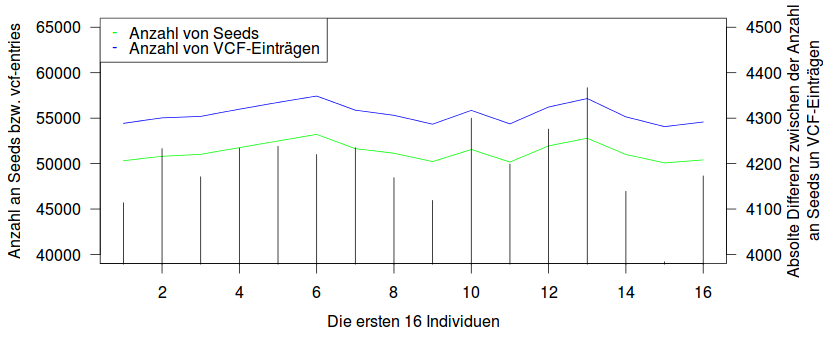
\includegraphics[width=0.9\linewidth]{figures/seedsVSvcf.png}}
\caption{\label{fig:seeds}\emph{Vergleich der Anzahl von Seeds gegen die zugrunde liegenden VCF-Einträge}. Der blaue Graph zeigt die Anzahl an Varianten der Referenzdatei des 1000 Genome Project. Der grüne Graph zeigt die entsprechende Anzahl an gefundenen Seeds als Ergebnis der Indexsuche. Die Indexsuche wurde mit dem Parameter $q=20$ und im Iterativen Schritt mit $q=15$ auf 16 Kernen durchgeführt, mit einer initialen Mindestgröße für Seeds von 100 . Die hinzugefügten Balken zeigen die absolute Differenz zwischen beiden Graphen. }
\end{figure}

\subsection{Leistung beim menschlichen Chromosoms 21}
\begin{table}[t]
\footnotesize
\centering{
\begin{tabular}{lccccccc}
\hline
\\
$\#$Chr 21 & Rohdaten & \multicolumn{3}{c}{Kompression auf Event-Ebene} & \multicolumn{3}{c}{Kompression auf JS-Ebene}\\
       &  & Vorher & Nachher & \textbf{Ratio} & Vorher & Nachher & \textbf{Ratio}\\
\hline
\\
10 &  573.72 &  7.24 &  2.29 & \textbf{250.16} & 12.93  &  7.28 & \textbf{78.82}\\
50 & 2659.97 & 36.08  & 7.02 & \textbf{378.94} & 64.19 &  34.83 & \textbf{76.38}\\
100 & 5215.63 & 71.68 & 12.77 & \textbf{408.56} & 127.49 &  69.03 & \textbf{75.55}\\
200 & 10431.27 & 144.08 & 24.69 & \textbf{422.50} & 256.47 & 139.53 & \textbf{74.76}\\
\\
\hline
\end{tabular}
}
\caption{\label{tab:space}\emph{Übersicht des Ergebnisse für das menschliche Chromosom 21}. Alle Angaben, bis auf die erste Zeile mit der Anzahl an Sequenzen, sind in Megabyte. Die Bezeichnung \textit{Vorher} bezieht sich hierbei auf das Ergebnis vor den in Sektion \ref{sec:evepro} beschriebenen Verbesserungen: Auf Event-Ebene vor der Zusammenführung und auf Journaled String (JS)-Ebene vor der Prozessierung. Das Verhältnis (Ratio) bezieht sich jeweils auf die \textit{'Nachher'}-Werte zu den entsprechenden Rohdaten.}
\end{table}

Der Kompressionsalgorithmus wurde auf einer verschiedenen Anzahl an menschlichen Chromosomen 21 getestet. Für alle 4 Datensätze (Anzahl 10,50,100 und 200 Sequenzen) wurden folgende Parametereinstellungen gewählt:\\

\begin{lstlisting}[style=BashInputStyle]
    $ compressFASTA -i input.fa -q 20 -q 15 -mss 100 -t 16 (-ev)
\end{lstlisting}

Auf den Parameter -$ev$ wurde zur Laufzeit- und Arbeitsspeicheranalyse verzichtet. 

Die resultierenden Ergebnisse sind in Tabelle~\ref{tab:space} aufgelistet. Es wird zwischen dem Speicheraufwand der eigentliche Speicherung einer Datei (Kompression auf Event-Ebene) und dem Arbeitsspeicheraufwand bei der Weiterverwendung mittels Journaled Strings (Kompression auf JS-Ebene) unterschieden.

Die generierten (vorher) und zusammengeführten (nachher) $\Delta$-Events können als solche in einer Datei gespeichert werden. Bisher wurde noch kein entsprechendes Ausgabeformat erstellt, weswegen die angegeben Werte hypothetischen Berechnungen entsprechen. Dabei werden für die Attribute $pos$, $type$ und $del$ jeweils ein \textit{unsigned integer} (4 Byte) und für den Bitvektor $seqs$ eine üngefähre Größe von $\#$Sequenzen/8 Byte (8 Bit pro Byte) berechnet. Der Wert für $ins$ wird bei der Ausgabe des Programms für jede Sequenz angegeben (vorrausgesetzt -$ev$ wurde spezifiziert). Es fällt auf, dass je mehr Sequenzen komprimiert werden, desto bessere Kompressionsverhältnisse werden erreicht. Die Verhältnisse sind mit denen anderer referentieller Algorithmen nur bedingt vergleichbar, da andere Datensätze verwendet wurden. [referenzen mit einem beispiel.].

Die Kompression auf Ebene der Journaled Strings erzielte geringere Verhältnisse. Es ist wichtig anzumerken, dass die Zusammenführung von Events keine Auswirkungen auf die Anzahl an Journal Entries hat, da jede Sequenz individuell und unabhängig aufgebaut werden muss. Daher entsprechen die Werte auch eher den 'Vorher'-Werten der Kompression auf Event-Ebene. Ein $\Delta$-Event ist prinzipiell mit einem Journal Entry gleichzusetzen. Zur Berechnung des Speicheraufwands eines Journaled Strings ............... .
Bei zunehmender Anzahl an Sequenzen singt das Kompressionsverhältnis in geringem Maße. Außerdem kann festgehalten werden, dass die Anzahl an Journal Entries mit Hilfe der Prozessierung um durchschnittlich die Hälfte reduziert wird, wodurch sich auch die der Speicherplatzverbrauch halbiert.

Laufzeit .... ?!

\subsection{Leistung bei E.Coli Genomen}

%%%%%%%%% CONCLUSION %%%%%%%%%%%%%%%%%%%%%%%%%%%%%%%%%%%%%%%%%%%%%%%%%%%%%%%%%%%
\section{Disskusion und Fazit}
\pagebreak
%%%%%%%%% REFERENCES %%%%%%%%%%%%%%%%%%%%%%%%%%%%%%%%%%%%%%%%%%%%%%%%%%%%%%%%%%%
%\bibliographystyle{apalike}  % Style
\bibliographystyle{acm}  % Style
\bibliography{myBibliography.bib}

\end{document}
